\documentclass[12pt]{article}
\usepackage{graphicx}
\usepackage{wrapfig}
\usepackage{xcolor}


\begin{document}
%\newpage
\pagecolor{black!83}
\pagenumbering{gobble}
\pagenumbering{roman}


\begin{titlepage}

\newcommand{\HRule}{\rule{\linewidth}{0.5mm}} 
\begin{center}

\includegraphics[width=100px, keepaspectratio]{10422078_1548897991993911_1856738101730602681_n}\\[1cm]
\textsc{\textbf{\textcolor{green}{\Large{Bangabandhu Sheikh Mujibur Rahman Science and Technology University}}}}\\[2cm]
\end{center}

\textsc{\Large \textcolor{teal}{Technical Writing and Presentation}}\\[0.5cm]
\HRule \\[0.4cm]
{ \huge \bfseries \textcolor{red}{ARTIFICIAL INTELLIGENCE}}\\[0.4cm] 
\HRule \\[1.5cm]
\begin{minipage}{0.4\textwidth}
\begin{flushleft} \large
\emph{\textcolor{white}{\Large Author:}}\\
\textcolor{brown}{Name :A.N.M.Tanvin Ahmed} \\\textcolor{brown}{Dept. of CSE} \\\textcolor{brown}{ID:18ICTCSE062} 
\end{flushleft}
\end{minipage}
~
\begin{minipage}{0.4\textwidth}
\begin{flushright} \large
\emph{\textcolor{white}{\Large Lecturer:}} \\
 \textcolor{brown}{Name : \textsc{Nasif Ahmed}\\\textcolor{brown}{Dept. of CSE}} \\
\end{flushright}
\end{minipage}\\[2cm]
{\large \textcolor{yellow}{ \today}}\\[.5cm] 
\end{titlepage}
\begin{center}
\begin{Huge}
\textbf{\textcolor{red}{Index}}\\
\end{Huge}
\end{center}
\begin{itemize}
\item[\textcolor{blue}{1.}] \textbf{\textcolor{blue}{Definition...............................................................ii}}
\item[\textcolor{blue}{2.}]\textbf{\textcolor{blue}{History...................................................................ii}}
\item[\textcolor{blue}{3.}]\textbf{\textcolor{blue}
{Classification of Artificial Intelligence...................iii}}
\begin{enumerate}
   \item[\textcolor{blue}{3.1.}]\textcolor{blue}{Reactive Machines.....................................................iii}
   \item[\textcolor{blue}{3.2.}]\textcolor{blue}{Limited Memory........................................................iv}
   \item[\textcolor{blue}{3.3.}]\textcolor{blue}{Theory of Mind.........................................................iv}
   \item[\textcolor{blue}{3.4.}]\textcolor{blue}{Self-awareness............................................................v}
\end{enumerate}
\item[\textcolor{blue}{4.}]\textbf{\textcolor{blue}{Some uses of Artificial intelligence.........................vi}}
\begin{enumerate}
   \item[\textcolor{blue}{4.1.}]\textcolor{blue}{Smart phones.............................................................vi}
   \item[\textcolor{blue}{4.2.}]\textcolor{blue}{Smart cars and Drones...............................................vi}
   \item[\textcolor{blue}{4.3.}]\textcolor{blue}{Social Media Feeds.....................................................vii}
   \item[\textcolor{blue}{4.4.}]\textcolor{blue}{Online Ads Network...................................................vii}
\end{enumerate}
\item[\textcolor{blue}{5.}]\textbf{\textcolor{blue}{The top myths about advanced AI........................viii}}
\item[\textcolor{blue}{6.}]\textbf{\textcolor{blue}{Scope of Artificial Intelligence...............................ix}}
\begin{enumerate}
   \item[\textcolor{blue}{6.1.}]\textcolor{blue}{Breakthrough in Science............................................ix}
   \item[\textcolor{blue}{6.2.}]\textcolor{blue}{Cyber Security...........................................................x}
   \item[\textcolor{blue}{6.3.}]\textcolor{blue}{Face Recognition........................................................xi}
   \item[\textcolor{blue}{6.4.}]\textcolor{blue}{Data Analysis.............................................................xi}
   \item[\textcolor{blue}{6.5.}]\textcolor{blue}{Transport....................................................................xii}\\\\\\\\\\\\\\\\\\\\\\
\end{enumerate}
\end{itemize}

                              

\begin{large}
\textbf{\textcolor{teal}{1.Definition :}}\\
\end{large}

\textcolor{white}{\textbf{\textcolor{yellow}{\huge C}}omputer science defines AI research as the study of "intelligent agents": any device that perceives its environment and takes actions that maximize its chance of successfully achieving its goals. A more elaborate definition characterizes AI as “a system’s ability to correctly interpret external data, to learn from such data, and to use those learnings to achieve specific goals and tasks through flexible adaptation.”}\\\\

\begin{figure}[h]
\centering
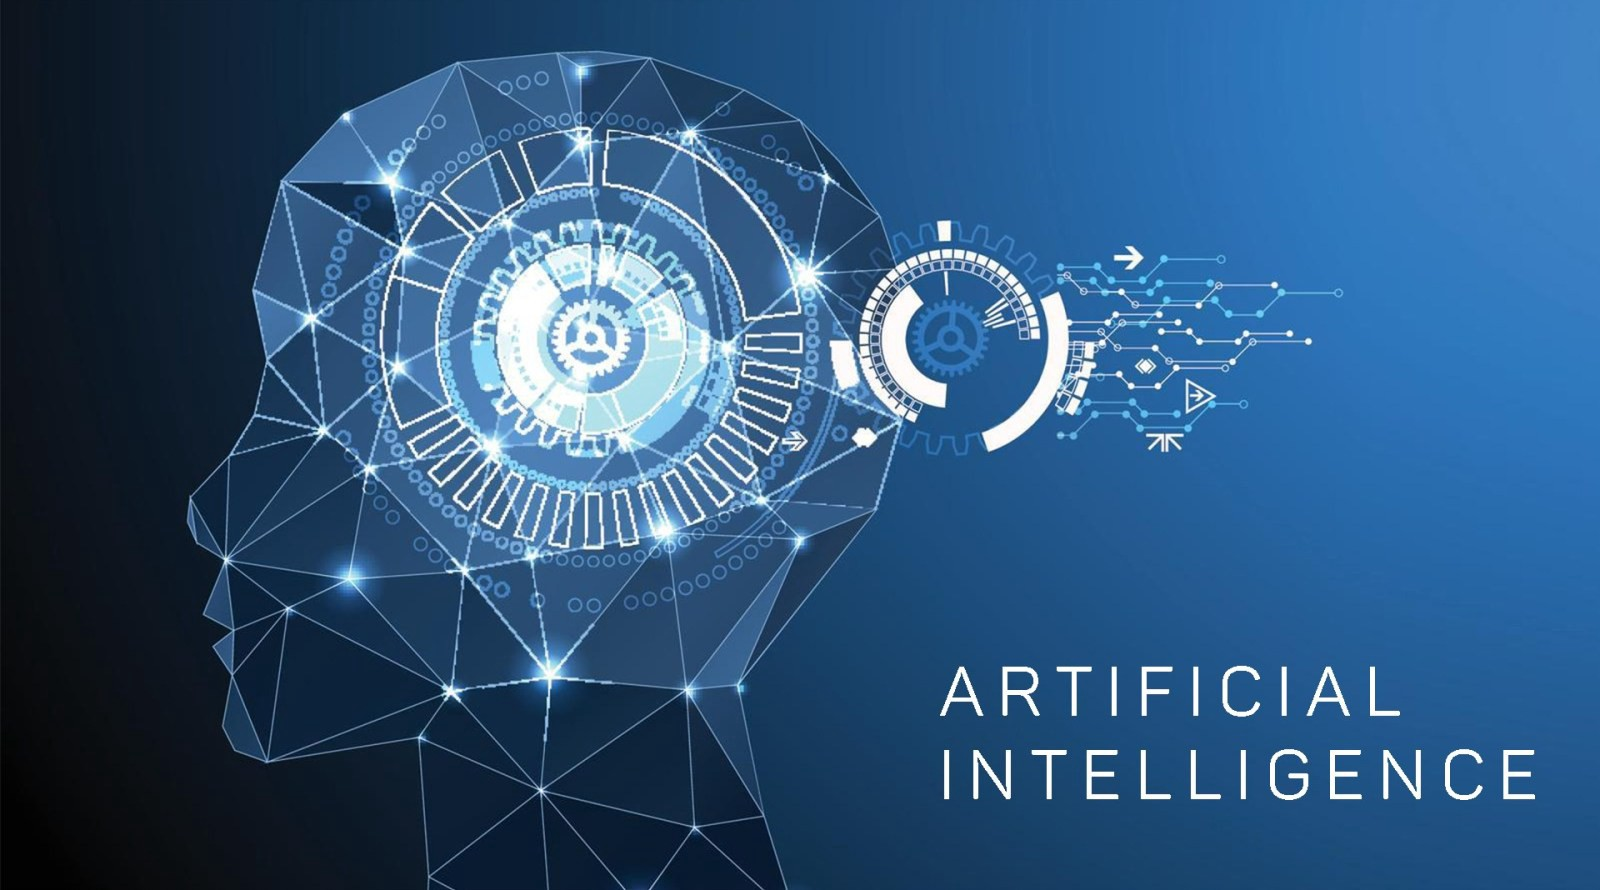
\includegraphics[scale=0.19]{1-thCB4VzqsRapqFCHC8w7EQ}
\caption{\textit{\textcolor{teal}{Artificial Intelligence}}}
\end{figure}

\begin{large}
\textbf{\textcolor{teal}{2.History :}}\\
\end{large}

\textcolor{white}{\textbf{\textcolor{yellow}{\huge T}}hought-capable artificial beings appeared as storytelling devices in antiquity,and have been common in fiction, as in Mary Shelley's Frankenstein or Karel Čapek's R.U.R. (Rossum's Universal Robots). These characters and their fates raised many of the same issues now discussed in the ethics of artificial intelligence.
According to Bloomberg's Jack Clark, 2015 was a landmark year for artificial intelligence, with the number of software projects that use AI Google increased from a "sporadic usage" in 2012 to more than 2,700 projects. Clark also presents factual data indicating the improvements of AI since 2012 supported by lower error rates in image processing tasks. He attributes this to an increase in affordable neural networks, due to a rise in cloud computing infrastructure and to an increase in research tools and datasets.Other cited examples include Microsoft's development of a Skype system that can automatically translate from one language to another and Facebook's system that can describe images to blind people. In a 2017 survey, one in five companies reported they had "incorporated AI in some offerings or processes". Around 2016, China greatly accelerated its government funding; given its large supply of data and its rapidly increasing research output, some observers believe it may be on track to becoming an "AI superpower". However, it has been acknowledged that reports regarding artificial intelligence have tended to be exaggerated.}\\\\


\begin{large}
\textbf{\textcolor{teal}{3.Classification of Artificial Intelligence :}} \\
\end{large}
\textcolor{white}{\textbf{\textcolor{yellow}{\huge T}}here are four types of artificial intelligence: reactive machines, limited memory, theory of mind and self-awareness.}\\\\


\begin{large}
\textbf{\textcolor{teal}{3.1. Reactive Machines :}}
\end{large}

\begin{wrapfigure}{r}{3in}
\centering
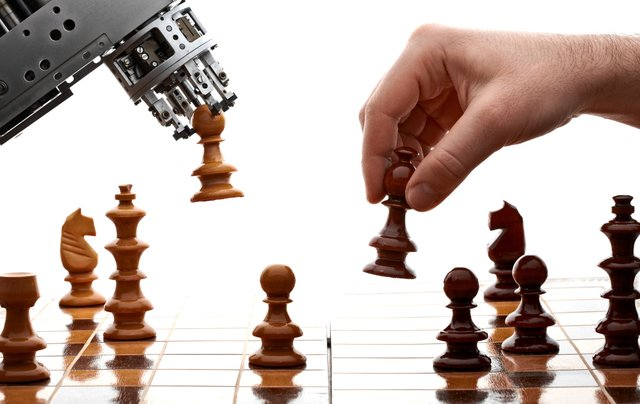
\includegraphics[width=2.9in]{AI-Paradigm-Need-For-AI-GoodWorkLabs}
\caption{\textit{\textcolor{teal}{Chess playing reactive machines.}}}
\end{wrapfigure}

\textcolor{white}{\textbf{\textcolor{yellow}{\huge T}}he most basic types of AI systems are purely reactive, and have the ability neither to form memories nor to use past experiences to inform current decisions. Deep Blue, IBM’s chess-playing supercomputer, which beat international grandmaster Garry Kasparov in the late 1990s, is the perfect example of this type of machine.}\\\\

\begin{large}
\textbf{\textcolor{teal}{3.2. Limited Memory :}}\\
\end{large}


\textcolor{white}{\textbf{\textcolor{yellow}{\huge T}}his Type II class contains machines can look into the past. Self-driving cars do some of this already. For example, they observe other cars’ speed and direction. That can’t be done in a just one moment, but rather requires identifying specific objects and monitoring them over time.
These observations are added to the self-driving cars’ preprogrammed representations of the world, which also include lane markings, traffic lights and other important elements, like curves in the road. They’re included when the car decides when to change lanes, to avoid cutting off another driver or being hit by a nearby car.
But these simple pieces of information about the past are only transient. They aren’t saved as part of the car’s library of experience it can learn from, the way human drivers compile experience over years behind the wheel.}

\begin{wrapfigure}{r}{3in}
\centering
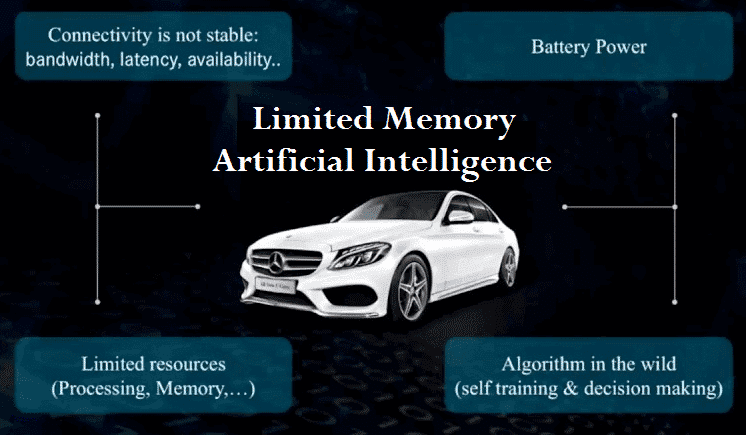
\includegraphics[width=3in]{5-Limited-Memory-Artificial-Intelligence}
\caption{\textit{\textcolor{teal}{A limited memory Artificial Intelligence.}}}
\end{wrapfigure}

\textcolor{white}{So how can we build AI systems that build full representations, remember their experiences and learn how to handle new situations? Brooks was right in that it is very difficult to do this. My own research into methods inspired by Darwinian evolution can start to make up for human shortcomings by letting the machines build their own representations.}\\

\begin{large}
\textbf{\textcolor{teal}{3.3. Theory of Mind :}}\\
\end{large}

\textcolor{white}{\textbf{\textcolor{yellow}{\huge W}}e might stop here, and call this point the important divide between the machines we have and the machines we will build in the future. However, it is better to be more specific to discuss the types of representations machines need to form, and what they need to be about.
Machines in the next, more advanced, class not only form representations about the world, but also about other agents or entities in the world. In psychology, this is called “theory of mind” – the understanding that people, creatures and objects in the world can have thoughts and emotions that affect their own behavior.
This is crucial to how we humans formed societies, because they allowed us to have social interactions. Without understanding each other’s motives and intentions, and without taking into account what somebody else knows either about me or the environment, working together is at best difficult, at worst impossible.
If AI systems are indeed ever to walk among us, they’ll have to be able to understand that each of us has thoughts and feelings and expectations for how we’ll be treated. And they’ll have to adjust their behavior accordingly.}\\\\

\begin{large}
\textbf{\textcolor{teal}{3.4. Self-awareness :}}\\
\end{large}

\textcolor{white}{\textbf{\textcolor{yellow}{\huge T}}he final step of AI development is to build systems that can form representations about themselves. Ultimately, we AI researchers will have to not only understand consciousness, but build machines that have it.}

\begin{wrapfigure}{r}{3in}
\centering
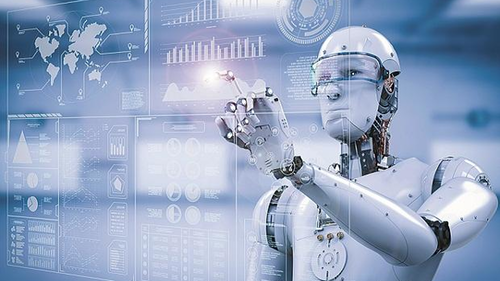
\includegraphics[width=3in]{self_aware_AI_26_Sept_2019.5d8d059954337}
\caption{\textit{\textcolor{teal}{Self aware AI.}}}
\end{wrapfigure}

\textcolor{white}{This is, in a sense, an extension of the “theory of mind” possessed by Type III artificial intelligences. Consciousness is also called “self-awareness” for a reason. (“I want that item” is a very different statement from “I know I want that item.”) Conscious beings are aware of themselves, know about their internal states, and are able to predict feelings of others. We assume someone honking behind us in traffic is angry or impatient, because that’s how we feel when we honk at others. Without a theory of mind, we could not make those sorts of inferences.
While we are probably far from creating machines that are self-aware, we should focus our efforts toward understanding memory, learning and the ability to base decisions on past experiences. This is an important step to understand human intelligence on its own. And it is crucial if we want to design or evolve machines that are more than exceptional at classifying what they see in front of them.}\\\\

\begin{large}
\textbf{\textcolor{teal}{4.Some uses of Artificial intelligence :}}\\
\end{large}
\textcolor{white}{\textbf{\textcolor{yellow}{\huge A}}I is one of the most helpful technology.Scientists are always think how it use in our daily uses technology.Some example are given below:}\\

\begin{large}
\textbf{\textcolor{teal}{4.1.Smart phones :}}\\
\end{large}

\begin{wrapfigure}{r}{3in}
\centering
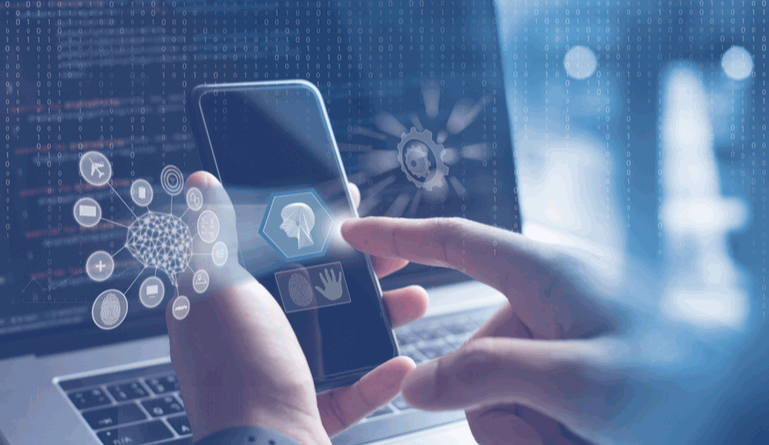
\includegraphics[width=3in]{Best-Practices-for-Integrating-AI-in-Mobile-App-Development-1}
\caption{\textit{\textcolor{teal}{AI in Smart Phone.}}}
\end{wrapfigure}

\textcolor{white}{\textbf{\textcolor{yellow}{\huge M}}ost manufacturers are now incorporating AI into their smartphones, with big chip manufacturers including Qualcomm and Huawei producing chips with built-in AI capabilities. AI integration can help bring features such as scene recognition, mixed and virtual reality elements, and more.}\\

\begin{large}
\textbf{\textcolor{teal}{4.2. Smart cars and Drones:}}\\
\end{large}

\textcolor{white}{\textbf{\textcolor{yellow}{\huge S}}peaking of AI, there is no better and more prominent demonstration of this technology than what smart car and drone manufacturers are doing with it. A few years ago, using a fully automatic car was a dream, but now that companies like Tesla have made so much progress, we already have a fleet of semi-automatic cars on the road.
Companies like Amazon and Walmart are investing heavily in drone delivery programs and this will become a reality sooner than you think. If you think this is too far, note that militaries around the world are already using successful drone programs.}\\\\\\\\\\\\\\\\\\\\\\


\begin{large}
\textbf{\textcolor{teal}{4.3. Social Media Feeds:}}\\
\end{large}
\begin{wrapfigure}{r}{3in}
\centering

\includegraphics[width=2.9in]{AI-Social-Media-800x470}

\caption{\textit{\textcolor{teal}{AI in Social Media.}}}
\end{wrapfigure}
\textcolor{white}{\textbf{\textcolor{yellow}{\huge I}}f you are thinking that smart cars will not affect you personally because they are not in your country or city, what you use on a regular basis. Even if you live under a rock, there is a high probability that you will tweet from under it. If Twitter isn't your poison choice, it could be Facebook or Instagram, or Snapchat, or any social media apps out there. Well, if you use social media, most of your decisions are influenced by artificial intelligence.}\\\\


\begin{large}
\textbf{\textcolor{teal}{4.4. Online Ads Network:}}\\
\end{large}

\textcolor{white}{\textbf{\textcolor{yellow}{\huge O}}ne of the biggest customers of Artificial Intelligence is the online advertising industry, which uses AI to track user statistics and serve our ads based on those statistics. Without AI, the online advertising industry would be failing because it would show random ads that consumers had no connection to their preferences. AI has been so successful in determining our interests and delivering advertising that the global digital ad industry has exceeded the US  250 billion US dolar, with the industry expected to exceed the 300 billion mark in 2019. So when you go online and see ads or a product recommendation, know that AI is affecting your life.}\\\\\\\\\\\\\\\\\\\\\\



\begin{large}
\textbf{\textcolor{teal}{5.The top myths about advanced AI :}}\\
\end{large}
\begin{wrapfigure}{r}{3in}
\centering
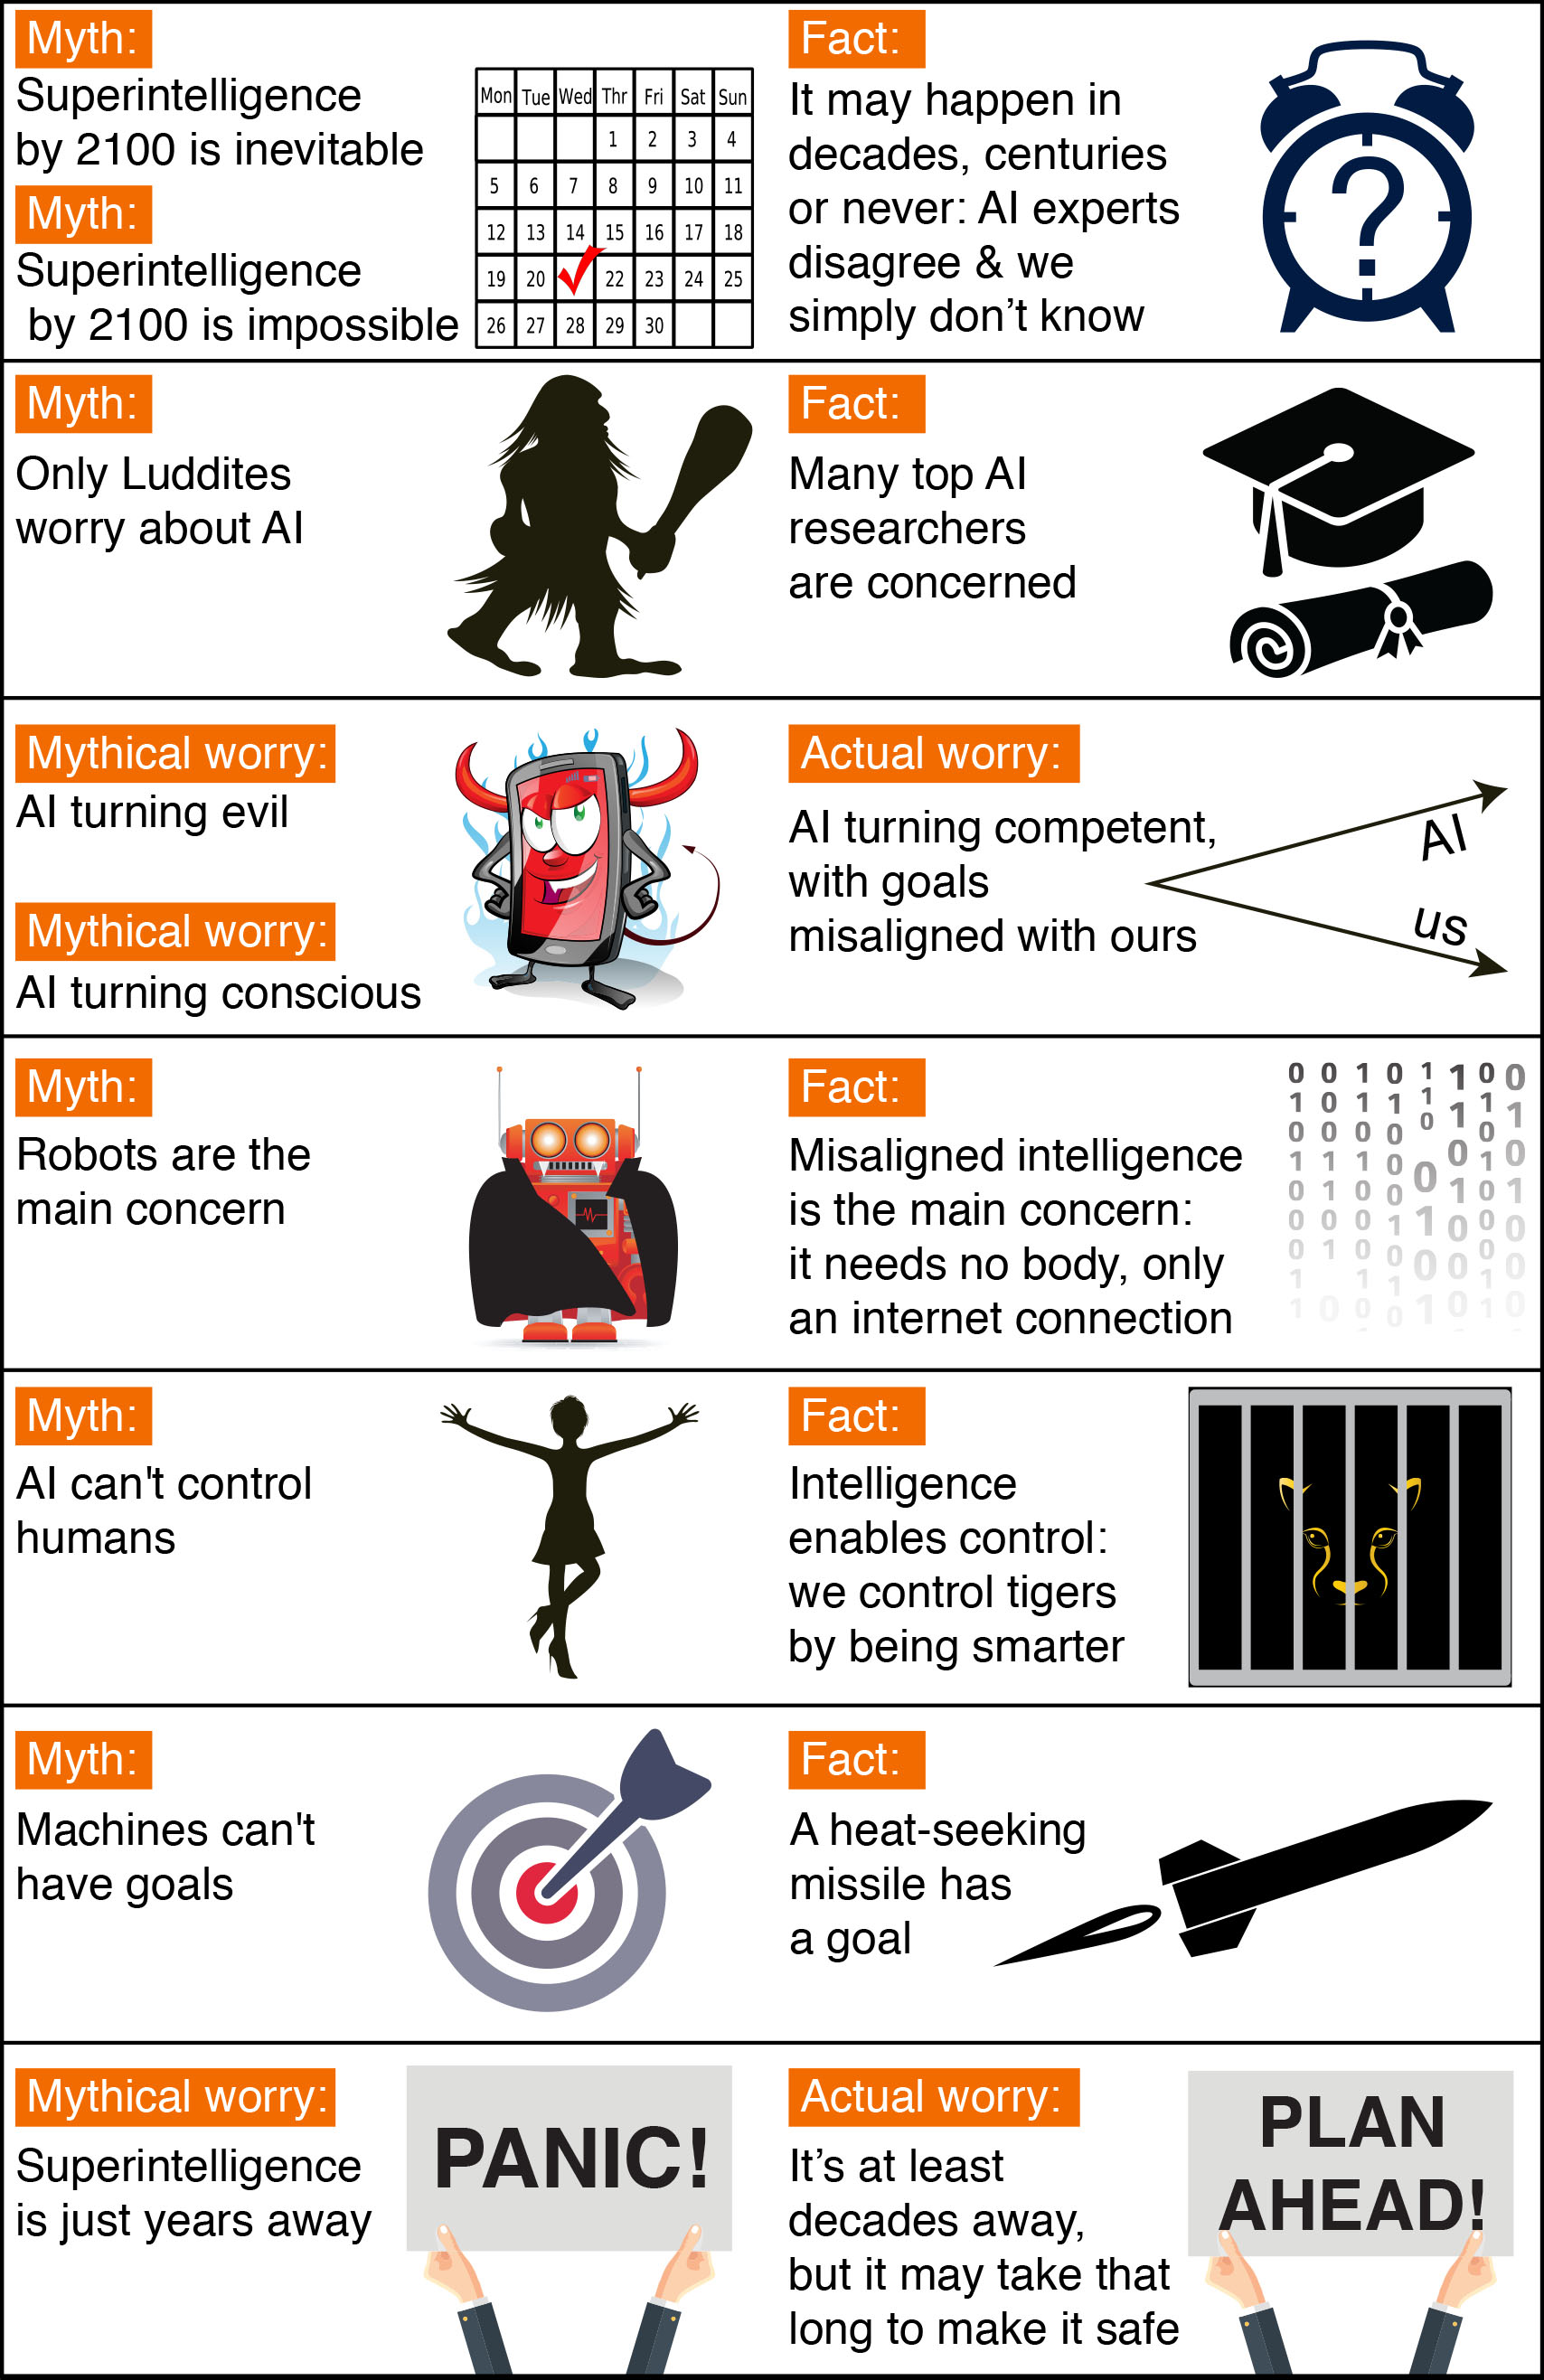
\includegraphics[width=2.9in]{myths-1}

\caption{\textit{\textcolor{teal}{most common myths.}}}
\end{wrapfigure}

\textcolor{white}{\textbf{\textcolor{yellow}{\huge A}} captivating conversation is taking place about the future of artificial intelligence and what it will/should mean for humanity. There are fascinating controversies where the world’s leading experts disagree,
 such as: AI’s future impact on the job market; if/when human-level AI will be developed; whether this will lead to an intelligence explosion; and whether this is something we should welcome or fear. But there are also many examples of of boring pseudo-controversies caused by people misunderstanding and talking past each other. To help ourselves focus on the interesting controversies and open questions — and not on the misunderstandings — let’s  clear up some of the most common myths.}\\\\\\\\\\\\\\\\
 
 \begin{large}
 \textbf{\textcolor{teal}{6.Future Scope of Artificial Intelligence :}}\\
 \end{large}
 
 \textcolor{white}{\textbf{\textcolor{yellow}{\huge A}}rtificial Intelligence(AI) is the simulation of human intelligence by machines. In other words, it is the method by which machines demonstrate certain aspects of human intelligence like learning, reasoning and self- correction. Since its inception, AI has demonstrated unprecedented growth. Sophia the AI Robot, is the quintessential example of this. The future of Artificial intelligence is hazy. But going by the bounds of progress AI has been making, it is clear AI will permeate every sphere of our life.}\\
 
 \begin{large}
 \textbf{\textcolor{teal}{6.1. Breakthrough in Science:}}\\
 \end{large}
 
\begin{wrapfigure}{r}{3in}
\centering
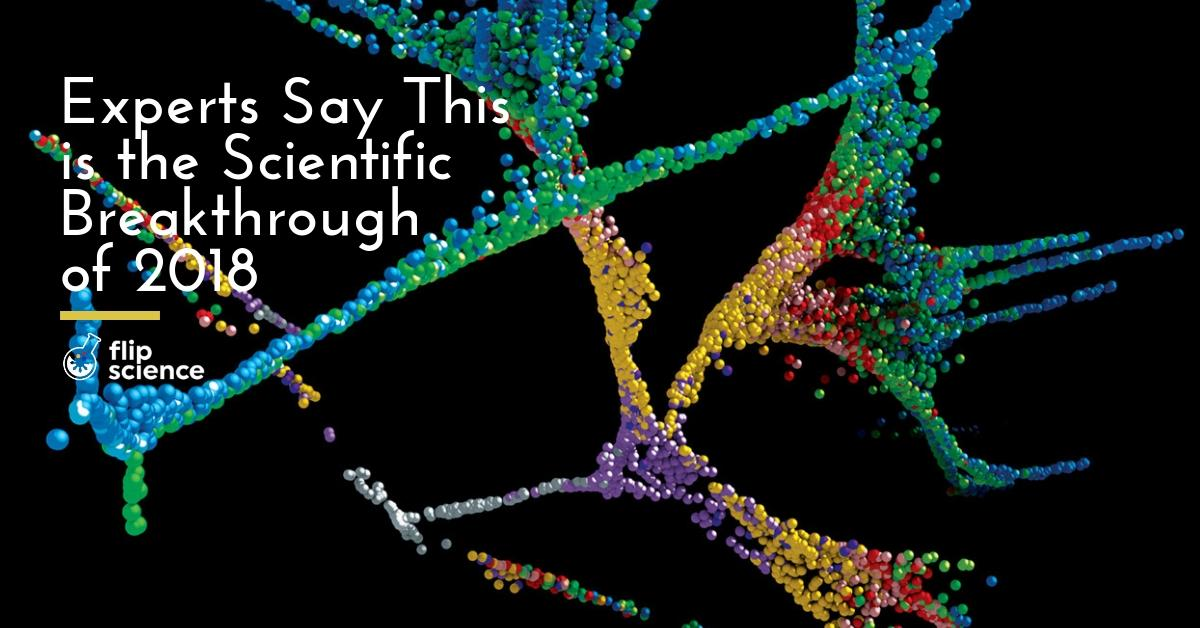
\includegraphics[width=2.9in]{FS.Covers.Dec2018-Jan2019-2-2}

\caption{\textit{\textcolor{teal}{Breakthrough in Science.}}}
\end{wrapfigure} 
 
\textcolor{white}{\textbf{\textcolor{yellow}{\huge T}}he scope of AI in science is the largest. Recently ‘Eve’ was in the news for discovering that an ingredient found commonly in toothpaste, is capable of curing Malaria. Here the subject in appreciation ‘Eve’ is not a human scientist, rather a Robot created by a team of scientists at the Universities of Manchester, Aberystwyth, and Cambridge.
Eve’s example hints at the possibility of AI playing a bigger role in science in future, not just merely for augmentation. AI will be able to create science, not merely do science as evidenced by the Robot Scientist, Eve. Automation using AI for drug discovery is a field that is rapidly growing, mainly because machines work faster than humans. AI is also being applied in related areas such as synthetic biology for the manufacture and rapid design of microorganisms for industrial uses. Taking all this in stride, AI is sure to transform science as we know it.}\\\\\\\\\\\\\\\\\\\\\\

\begin{large}
\textbf{\textcolor{teal}{6.2. Cyber Security:}}\\
\end{large}

\begin{wrapfigure}{r}{3in}
\centering
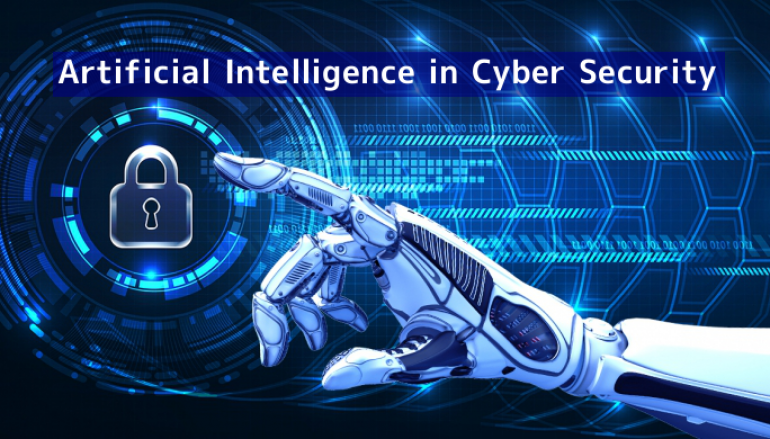
\includegraphics[width=2.9in]{rgOcI1557207528-770x439_c}

\caption{\textit{\textcolor{teal}{AI in Cyber Security.}}}
\end{wrapfigure}

\textcolor{white}{\textbf{\textcolor{yellow}{\huge T}}he future application of AI in cybersecurity will ensure in curbing hackers. The incidence of cybercrime is an issue that has been escalating through the years. It costs enterprises in term of brand image as well as material cost. Credit card fraudery is one of the most prevalent cybercrimes. Despite there being detection techniques, they still prove to be ineffective in curbing hackers. AI can bring a remarkable change to this. Novel AI techniques like Recurrent Neural Networks can detect fraudery in initial stages itself. This fraud detection system will be able to scan thousands of transactions instantly and predict/ classify them into buckets. RNN can save a lot of time as it focuses on cases where there is a high probability for fraud.}\\\\\\\\[2cm]

\begin{large}
\textbf{\textcolor{teal}{6.3. Face Recognition:}}\\
\end{large}

\begin{wrapfigure}{r}{3in}
\centering
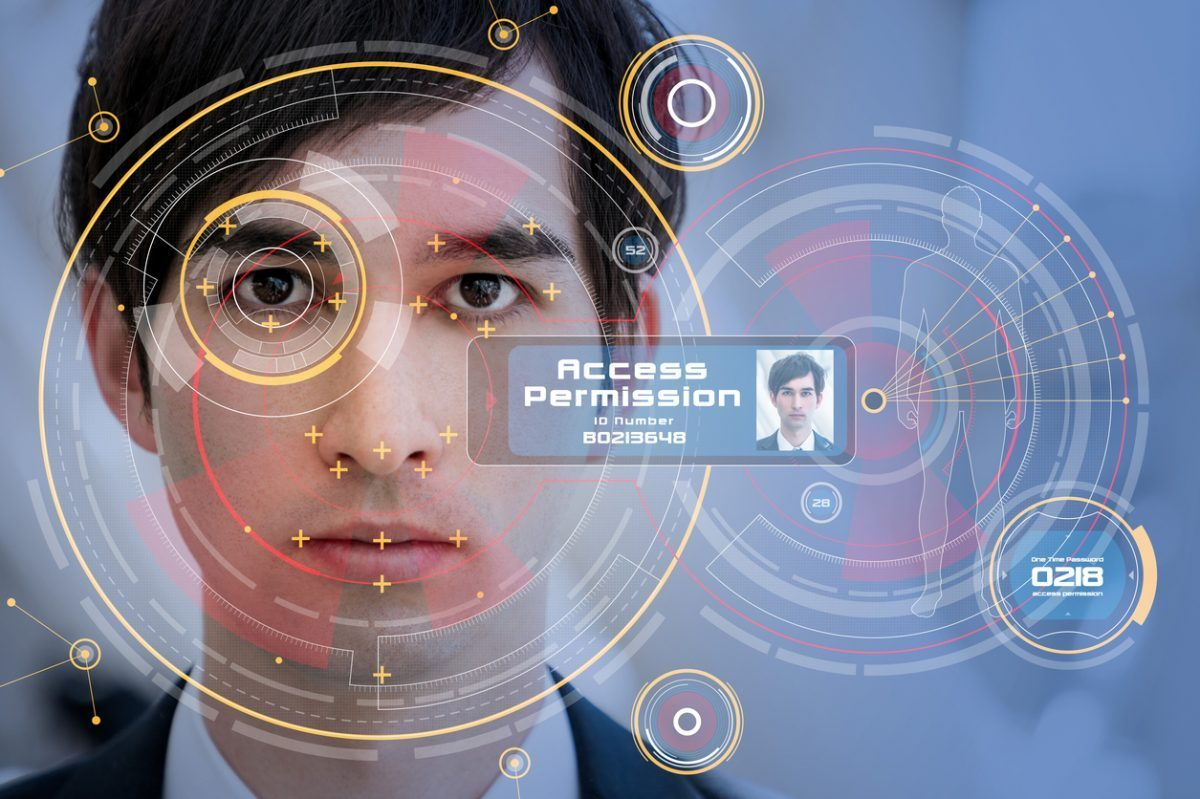
\includegraphics[width=2.9in]{russia-startup-facial-recognition-ethnicity}

\caption{\textit{\textcolor{teal}{AI in Face Recognetion.}}}
\end{wrapfigure}

\textcolor{white}{\textbf{\textcolor{yellow}{\huge T}}he launch of iPhone x with face recognition feature was a step towards AI future. In the coming years,
 iPhone users might be to unlock their phones by looking into the front camera. Authenticating personal content is not the only use of facial recognition. Governments and security forces make use of this feature to track down criminals and identify citizens. In the future, facial recognition can go beyond physical structure to emotional analysis. For example, it might become possible to detect whether a person is stressed or angry.}\\

\begin{large}
\textbf{\textcolor{teal}{6.4. Data Analysis:}}\\
\end{large}
\textcolor{white}{\textbf{\textcolor{yellow}{\huge O}}ne of the ways AI will benefit business is in the field of Data Analysis. AI would be able to perceive patterns in data that humans cannot. This enables business’ to target the right customers for the product. An example of this is the partnership between IBM and Fluid. Fluid, a digital retail company uses Watson – an AI created by IBM for insightful product recommendation to its customers.}\\[5cm]

\begin{large}
\textbf{\textcolor{teal}{6.5. Transport:}}\\
\end{large}

\begin{wrapfigure}{r}{3in}
\centering
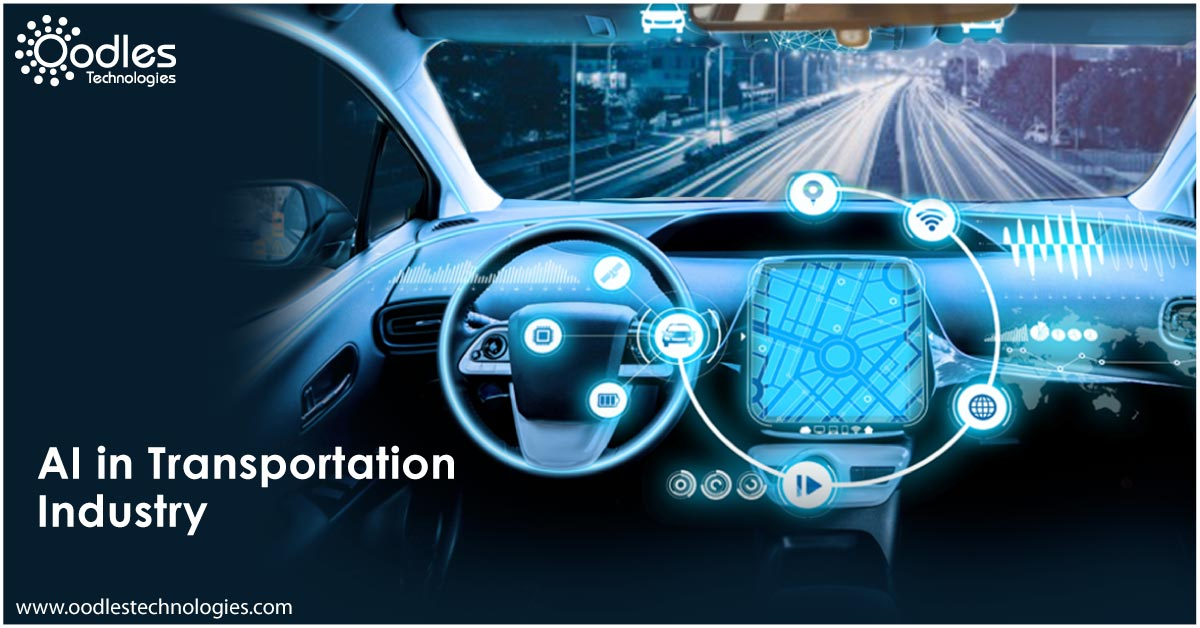
\includegraphics[width=2.9in]{d1acc567-5be1-4738-9b8e-663b8d182bfa}

\caption{\textit{\textcolor{teal}{AI in Transportation.}}}
\end{wrapfigure}
\textcolor{white}{\textbf{\textcolor{yellow}{\huge A}}I-guided transport will no longer be confined to the pages of sci-fi literature. Self- driving cars have already populated the market, however, a driver is required at the wheels for safety purposes. With Google, Uber and General Motors trying to establish themselves at the top in this market, it will not be long before driverless vehicles become a reality. Machine Learning will be crucial in ensuring that these Automated Vehicles operate smoothly and efficiently.}\\

\end{document}